% Relatório  para Disciplina de Controle Fuzzy - UFRN
% Autores:

%   FERNANDO LEANDRO FERNANDES
%   ROSENILDO PEREIRA AGUIAR FURTADO
%   TIAGO BATISTA SILVA SOUSA 

%%%%%%%%%%%%%%%%%%%%%%%% STRUCTURE %%%%%%%%%%%%%%%%%%%%%%%%%%
\documentclass[a4paper,12pt]{article}
\usepackage[T1]{fontenc}
\usepackage[utf8]{inputenc} 
\usepackage[brazil]{babel}
\usepackage{lmodern}
\usepackage{setspace}
\usepackage[top=2cm, bottom=2cm, left=2cm, right=2cm]{geometry}
\usepackage{indentfirst} 

\setcounter{section}{0}

%%%%%%%%%%%%%%%%%%%%%%%%%%%% PAGES STYLE %%%%%%%%%%%%%%%%%%%%%
\usepackage{fancyhdr}
\fancypagestyle{main}{
\renewcommand{\headrulewidth}{0pt}
\fancyhead[RO]{\thepage}
\fancyfoot[CO]{}
}
%%%%%%%%%%%%%%%%%%%%%%  PACOTES  %%%%%%%%%%%%%%%%%%%%%%%%%%%%

\usepackage{graphicx}
\usepackage{epstopdf}
\usepackage{subfig}
\usepackage[titles,subfigure]{tocloft}
\usepackage{mathptmx}
\usepackage{changepage}
\usepackage{amsmath}
%\usepackage[alf]{abntex2cite}
\usepackage{booktabs}
\usepackage{textcomp}

%%%%%%%%%%%%%%%%%%%%%%% PDF METADATA %%%%%%%%%%%%%%%%%%%%%%%%%

\usepackage[ pdftitle={3 Relatório fuzzy},
pdfsubject={OTIMIZACAO_NUMERICA},
pdfkeywords={Controle,Automação,UFRN,DCA,ipump},
hidelinks]{hyperref}

\renewcommand\thesection{\arabic{section}}


%%%%%%%%%%%%% Criando novo tipo de lista %%%%%%%%%%%%%%%%%%%%%%
% http://texblog.org/2008/07/13/define-your-own-list-of/

\newcommand{\listexamplename}{Lista de Equações}
\newlistof{equacao}{exp}{\listexamplename}
\newcommand{\equacao}[1] {%
    \refstepcounter{equacao}
    \par\noindent\begin{center}\textbf{Equação \theequacao. #1}\end{center}
    \addcontentsline{exp}{equacao}
        {\protect\numberline{\thesection.\theequacao}\quad#1}\par
}

%%%%%%%%%%%%%%%%%%%%%%%%%%%%%%%%%%%%%%%%%%%%%%%%%%%%%%%%%%%%%%%%%

\begin{document}

\onehalfspacing

\thispagestyle{empty}

\setcounter{page}{1}

%%%%%%%%%%%%%%%%%%%%%%% LOGOS %%%%%%%%%%%%%%%%%%%%%%%%%%%%%%%

\begin{figure}[!ht]

\centering

\subfloat{

\includegraphics[width=2.7cm]{UFRN-brasao.jpg}
\label{UFRN Logo}
}
\vspace{1cm}

%\caption{}
\label{Logos}

\end{figure}

%%%%%%%%%%%%%%%%%%%%%%%%%%% CAPA %%%%%%%%%%%%%%%%%%%%%%%%%%%%%

\vspace{-1cm}

\begin{center}
{\bf{\normalsize UNIVERSIDADE FEDERAL DO RIO GRANDE DO NORTE\\
CENTRO DE TECNOLOGIA\\
DEPARTAMENTO DE ENGENHARIA DE COMPUTAÇÃO E AUTOMAÇÃO\\
CURSO DE ENGENHARIA MECATRÔNICA
}}


\vspace{5cm}

{\bf{\large RELATÓRIO DA 3º UNIDADE DE \\CONTROLE FUZZY DE SISTEMAS DINÂMICOS\\
OTIMIZAÇÃO NUMÉRICA\\
}}


\vspace{2.6cm}



\begin{flushright}
\begin{normalsize}
FERNANDO LEANDRO FERNANDES (20150146106)\\
\vspace{0.8cm}
ROSENILDO PEREIRA AGUIAR FURTADO (20150146554)\\
\vspace{0.8cm}
TIAGO BATISTA SILVA SOUSA (20150146198)\\
\end{normalsize}
\end{flushright}


\vspace{3.6cm}
{\large Natal-RN\\
2016}
\end{center}


\newpage

%%%%%%%%%%%%%%%%%%%%%%%%%%%  CONTRA-CAPA %%%%%%%%%%%%%%%%%%%%%

\thispagestyle{empty}

\begin{center}
\begin{normalsize}
FERNANDO LEANDRO FERNANDES (20150146106)\\
\vspace{0.8cm}
ROSENILDO PEREIRA AGUIAR FURTADO (20150146554)\\
\vspace{0.8cm}
TIAGO BATISTA SILVA SOUSA (20150146198)\\


\end{normalsize}
\end{center}
\vspace{6cm}

{\bf{\large {\centering RELATÓRIO DA 3º UNIDADE DE \\ CONTROLE FUZZY DE SISTEMAS DINÂMICOS\\
OTIMIZAÇÃO NUMÉRICA\\}}}

\vspace{2cm}

\begin{adjustwidth}{7.5cm}{0cm}

{\normalsize

Terceiro Relatório apresentado à disciplina de
Controle Fuzzy de Sistemas dinâmicos, correspondente à
avaliação da 3º unidade do semestre 2016.2 do 9º período
do curso de Engenharia Mecatrônica da
Universidade Federal do Rio Grande do Norte, sob
orientação do mestrando {\bf Eng. Alcemy Gabriel Vitor Severino.}

}

\end{adjustwidth}

\vspace{1.5cm}

\begin{center}

Professor {\bf Dr. Fábio Meneghetti Ugulino de Araújo}.

\vspace{3.5cm}

{\large Natal-RN\\
2016}

\end{center}

\newpage

%%%%%%%%%%%%%%%%%%%%%%%%%%%  RESUMO %%%%%%%%%%%%%%%%%%%%%%%%%%

\thispagestyle{empty}

\begin{center}
{\large \textbf{RESUMO}}
\end{center}

\vspace{2cm}

Esta atividade é componente do conjunto de avaliações da 3a. unidade da disciplina Controle \emph{Fuzzy} de Sistemas Dinâmicos (DCA0126), do período 2016.2, do curso de Engenharia Mecatrônica da Universidade Federal do Rio Grande do Norte. 

O presente relatório descreve métodos de otimização numérica(maximização ou minimização) de funções bidimensionais utilizando os métodos ``algoritmo genético'' e ``otimização por enxame de partículas''. Os algoritmos de otimização foram implementados no MATLAB R2014a e aplicados a algumas das funções disponíveis no site  \textit{Virtual Test Functions and Datasets} diponível no \emph{site} \url{http://www.sfu.ca/~ssurjano/optimization.html} (acesso em 29 de novembro de 2016).

\vspace{1cm}

\textbf{Palavras-chave}: \textit{Otimização Numérica, Algoritmo Genético, GA, Enxame de partículas, PSO.}

\newpage


%%%%%%%%%%%%%%%%%%%%% LISTA DE FIGURAS %%%%%%%%%%%%%%%%%%%%%%%

\thispagestyle{empty}

\begin{center}
\listoffigures
\end{center}

\newpage

%%%%%%%%%%%%%%%%%%%%% LISTA DE equações %%%%%%%%%%%%%%%%%%%%%%%

\thispagestyle{empty}
\newcommand{\listequationsname}{\begin{center}Lista de Equações\end{center}}
\newlistof{myequations}{equ}{\listequationsname}
\newcommand{\myequations}[1]{%
\addcontentsline{equ}{myequations}{\protect\numberline{\theequation}#1}\par}


%%%%%%%%%%%%%%%%%%%%%%%%%%% SUMÁRIO %%%%%%%%%%%%%%%%%%%%%%%%%%

\thispagestyle{empty}

\begin{center}
\tableofcontents
\end{center}

\newpage

%%%%%%%%%%%%%%%%%%%%%%%%%%% INTRODUÇÃO %%%%%%%%%%%%%%%%%%%%%%%

\thispagestyle{main}

\section{Introdução}

Os métodos de otimização numérica consistem algoritmos de busca iterativa por pontos de máximo ou mínimo de funções nas quais a aplicação de métodos analíticos é ineficiente, custosa ou mesmo impraticável.

Os algoritimos numéricos para solução de problemas de otimização são essencialmente classificados em métodos de programação matemática e métodos probabilísticos. A diferença essencial dos métodos de programação matemática para os métodos probabilísticos é que os últimos procuram encontrar o mínimo global do problema de otimização evitando os mínimos locais. Já os métodos de programação matemática fornecem um mínimo local. 

Os métodos probabilísticos, como o próprio nome sugere, se utilizam de um processo de busca randômica guiados por decisões probabilísticas para obter o mínimo global. Além disso, os métodos probabilísticos são também ferramentas poderosas para problemas com variáveis discretas. 

Dentre os métodos probabilísticos existentes, destacam-se o método do algoritmo genético (\emph{genetic algorithm -- GA)}, que simula a evolução biológica natural das espécies para procurar o indivíduo (possível solução) com a melhor adaptação e o enxame de partículas (\emph{particle swarm optimization -- PSO}). 

Para casos de minimização, a adaptação de cada indivíduo é calculada como o inverso do valor da função a ser otimizada em cada indivíduo, que é representado por um par ordenado bidimensional.

Nesta atividade exploraremos especificamente o algoritmo genético e o enxame de partículas na determinação de mínimos e máximos de funções exóticas.

\newpage

%%%%%%%%%%%%%%%%% REFERENCIAL TEÓRICO %%%%%%%%%%%%%%%%%%%%%%

\thispagestyle{main}

\section{Referencial Teórico}

Apresentamos a seguir os conceito envolvidos na teoria dos algoritmos de otimização numérica implementados nesta atividade, especialmente o algoritmo genético e algoritmo de otimização por enxame de partículas. 

\subsection{Algoritmo Genético}

A classe de algoritmos denominados genéticos (ou GA, do inglês \textit{genetic algorithm}) consistem em uma mimetização do processo evolucionário das espécies \cite{Linden:2008}, basicamente, pela reprodução do processo de evolução biológica das espécies para otimizar problemas diversos, incluindo problemas matemáticos. 

O algoritmo teve seu início na primeira metade da década de 1950, resultado do trabalho do matemático norueguês-italiano Nills Aall Barricelli, em Princeton, New Jersey \cite{KennedyEberhart:1995}. Apesar de sua publicação ser de 1954, os fundamentos do algoritmo genético não entraram em evidência até os anos 1960, quando o seu estudo foi vastamente difundido. Também nos anos 1950, o inglês Alex Fraser publicou uma série de artigos sobre o assunto, por exemplo \cite{Fraser:1957} e \cite{Fraser_etal:1970}. Genericamente, o algoritmo gera uma população aleatória e com o passar das gerações, a população converge para uma solução de mínimo/máximo global.

Os algoritmos genéticos são técnicas probabilísticas que manipula um conjunto numeroso de indivíduos (população), sendo uma heurística de busca no espaço de estados. Assim, mesmo com uma população inicial e parâmetros de configuração idênticos, é provável que sejam encontrados resultados diferentes ainda que convergentes a um valor comum.


\subsubsection{Representação dos indivíduos}

Cada indivíduo é representado por $n$ valores, onde $n$ é a dimensão de entrada da função-problema. Esses valores podem ser utilizados nas bases binária ou decimal. Os indivíduos têm um "valor de adaptação ao meio", que é chamado de adaptação que representa o quão próximo da solução aquele indivíduo está. Para casos de maximização, a adaptação é igual ao valor da função naquele ponto (indivíduo), para minimização, o inverso do valor da função avaliada no ponto. O algoritmo selecionará quais indivíduos passarão seus genes para as próximas gerações através dos métodos de seleção descritos na subseção \ref{metodo-selecao}. 

\subsubsection{Métodos de seleção}
\label{metodo-selecao}

As GAs, diferentemente das buscas aleatórias (\emph{ramdom walk}), são buscas orientadas por informações pertinentes ao problema que direcionam sua busca através do mecanismo de seleção, novamente, assemelhado ao processo natural. Alguns métodos de seleção propostos para cumprir o papel da escolha dos melhores indivíduos segundo algum critério de avaliação e que, em tese, estariam mais aptos a otimizar o problema proposto. 

A seguir são apresentados alguns desses métodos:

\begin{itemize}

\item \textbf{ROLETA}: O método da roleta consiste em selecionar o indivíduo baseado na sua adaptação em relação à população total. Dessa forma, o indivíduo(solução) mais adaptado terá uma maior probabilidade de passar no teste e gerar filhos.

\item \textbf{TORNEIO}: O método do torneio seleciona apenas os melhores indivíduos, ou seja, aqueles pontos que estão mais próximos da solução desejada(mínimo ou máximo). Ele é particularmente eficiente em funções que possuem poucos ou nenhum mínimo local.

\item \textbf{SORTEIO}: O método do sorteio seleciona aleatoriamente indivíduos na população sem levar em conta a sua adaptação. Por não ser consistente, esse método não é muito utilizado.

\end{itemize}

\subsubsection{Cruzamento}
\label{cruzamento}

Após a subpopulação de pais ser definida pela aplicação de um dos métodos descritos, o cruzamento (troca de material genético) entre os indivíduos selecionados como pais, será realizado nos pares de cromossomos(no caso $x_1$ e $x_2$). Para que isso ocorra, será selecionado um número aleatório que representa a parte de material genético (coordenadas $x_1$ e $x_2$) que cada filho herdará de seus pais. 

Técnicas de cruzamento:

\begin{itemize}

\item Cruzamento na base binária: Neste cruzamento (cruzamento binário), cada indivíduo é representado por $n$ palavras de $m$ bits e a troca de material genético é feita sorteando um número inteiro, chamado de $flag$, que representa quantos bits de cada parâmetro do indivíduo pai serão mesclados com o restante de bits do indivíduo mãe. Isto é, se $m$ = 8 e $flag$ = 3, os 3 primeiros bits do pai e os 5 últimos bits da mãe serão usados para gerar um filho, e os bits restantes são utilizados para gerar o segundo filho.

\item Cruzamento na base decimal: De forma semelhante, o cruzamento na base decimal (cruzamento decimal) é feito atribuindo um valor de $flag$ percentual e aplicando o mesmo raciocínio do cruzamento binário ao valor decimal dos pais para gerar os filhos.
\end{itemize}

\subsubsection{Mutação}

O técnica de mutação é utilizada para gerar um indivíduo com características diversa em relação ao resto da população. Isso é feito com intuito de adicionar algum nível de aleatoriedade ao processo e, assim, evitar que o algoritmo fique confinado em um mínimo local.


\subsubsection{Fluxograma}

O fluxograma do algoritmo genético é o apresentado na figura \ref{fig:fluxo-ga}.
\begin{figure}[htb]
\begin{center}
    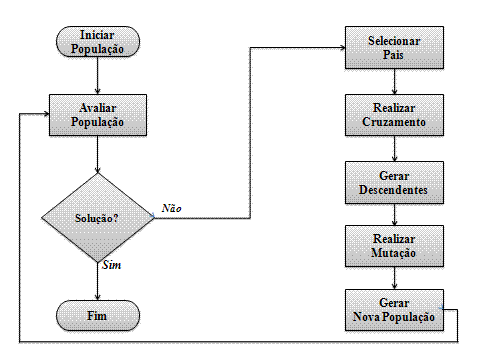
\includegraphics[scale=0.5]{fluxo-ga.png}
    \caption { Fluxograma do algoritmo genético. }
	\label{fig:fluxo-ga}
\end{center}
\end{figure}
\newpage
\subsection{Enxame de partículas}

A técnica de otimização por enxame de partículas, do inglês \textit{particle swarm optimization (PSO)}, foi concebida pelos sócio-psicólogo James Kennedy e pelo engenheiro eletricista Russel Eberhart, ambos americanos, inspirada no comportamento de uma revoada de pássaros, e seu primeiro intuito era o estudo em experimentos sociais \cite{KennedyEberhart:1995}. A otimização é feita através da aplicação de uma população de partículas e que são movidas no espaço de entrada da função à procura de uma solução de máximo ou mínimo.

A categoria de algoritmos computacionais de otimização por enxame de partículas são caracterizados pela forma iterativa que usam para  melhorar uma partícula-solução tendo como métrica a própria função a ser otimizada \cite{Yang_etal:2013}. Esses algorítimos fazem parte da família de algoritmos que aplicam inteligência de enxame \emph{swarm intelligence}. 

\subsubsection{O algoritmo}

Como mencionado anteriormente, o enxame de partículas simula o comportamento de uma revoada de pássaros. Ele usa o que aprende do cenário e o usa para resolver os problemas de otimização. No PSO cada solução, ou partícula, é um "pássaro" no espaço de solução. Todas as partículas tem valores de \emph{fitness} que são calculadas da função a ser otimizada e tem velocidades que direcionam o "voo" das partículas. As partículas se movem pelo espaço do problema seguindo as partículas ótimas encontradas.

O algoritmo é inicializado com um grupo de partículas (soluções) aleatórias e, a partir daí, busca pela solução ótima atualizando as gerações. Em cada iteração, cada partícula é atualizada pela melhor solução (\emph{fitness}) que ela alcançou, denominada \emph{pbest}, assim como o melhor solução entre todas apresentadas pelo enxame, o \emph{gbest}, conforme a equação \ref{eq:velocidade-pso}.

\newpage
\begin{equation}
    v_p[^.] = w * v_p[^.] + c1 * rand() * (\emph{pbest}[^.] - p[^.]) + c2 * rand() * (\emph{gbest} - p[^.])
\label{eq:velocidade-pso}
\end{equation}

\begin{equation}
	p[^.] = p[^.] + v_p[^.]
\label{eq:particula-pso}
\end{equation}
\\
 onde $w$ é a inércia da partícula, $v_p$ é a velocidade da particula, $c_1$ e $c_2$ são constantes de aprendizado e $p$ é a própria particula.

Desta forma, são considerados tanto a contribuição individual de cada elemento em separado, como o resultado coletivo do enxame.

\subsubsection{Fluxograma}

O fluxograma do algoritmo do enxame de partículas é o apresentado na figura \ref{fig:fluxo-pso}.
\begin{figure}[htb]
\begin{center}
    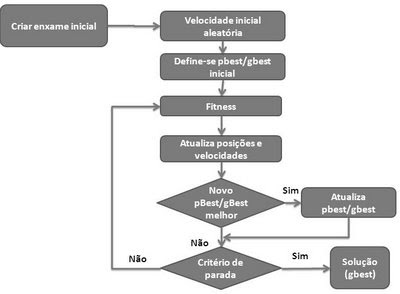
\includegraphics[scale=0.8]{fluxo-pso.jpg}
    \caption { Fluxograma do algoritmo do enxame de partículas. }
	\label{fig:fluxo-pso}
\end{center}
\end{figure}

\subsection{Comparação entre GA e PSO}

Ambas as técnicas, GA e PSO, seguem o procedimento abaixo:

\begin{enumerate}
\item Geração aleatória de uma população inicial
\item Cômputo do \emph{fitness} para cada indivíduo. Isso dependerá da distância para o objetivo
\item Reprodução da população com base nos valores de \emph{fitness} de cada indivíduo
\item Se os objetivos foram alcançados, então pare. Se não, volte ao passo 2.
\end{enumerate}

Do procedimento acima podemos afirmar que o PSO compartilha várias características com o GA. Ambos iniciam com uma população gerada aleatoriamente, ambos tem valores de aptidão (\emph{fitness}) para avaliar a população. Ambos atualizam a população e buscam pelo valor ótimo com técnicas ramdômicas. Nenhum dos algoritmos garante sucesso.

Entretanto, o PSO não tem operações "genéticas" como cruzamento e mutação. Nele, as partículas atualizam a si mesmas com a velocidade interna. Elas também tem memória, característica importante do algoritmo.

%\newpage
%%%%%%%%%%%%%%%%%%%%%% METODOLOGIA %%%%%%%%%%%%%%%%%%%%%%%%%%

\thispagestyle{main}

\section{Metodologia}

A implementação dos algoritmos de otimização apresentados neste relatório foi desenvolvida em \textit{scripts} da ferramenta de simulação MATLAB \cite{Moore:2012}, versão R2014a.

Os testes de execução foram realizados 100 vezes para cada função e algoritmo. Para cada caso foram calculados a mediana, menor e maior valor da posição do indivíduo/agente e o desvio-padrão dos valores da função (solução) obtidos para que ser averiguasse a convergência dos resultados apresentados.
 
\subsection{Funções para otimização}

As funções escolhidas para realizar otimização foram retiradas do site \textit{Virtual Test Functions and Datasets}\footnote{\url{ http://www.sfu.ca/~ssurjano/optimization.html}, acesso em 29 de novembro de 2016}. As funções escolhidas são apresentadas a seguir.


\subsubsection{Função \textit{Bukin} no. 6}

A sexta função \textit{Bukin} possui diversos mínimos locais, todos recaem em uma fenda. A expressão da função é a apresentada pela equação \ref{eq:bukin6}.

\begin{equation}
	f(x) = 100 \sqrt{|x_2 - 0.01x_1^2|} + 0.01 |x_1 + 10|
\label{eq:bukin6}
\end{equation}
\\
cujo domínio de entrada é dado pelo retângulo $x_1 \in [-15, 5]$, $x_2 \in [-3, 3]$ e tem mínimo global em $f(x^*) = 0$, para $x^* = (-10, 1)$.

O gráfico da função é o apresentado na figura \ref{fig:bukin6}.
\begin{figure}[htb]
\begin{center}
    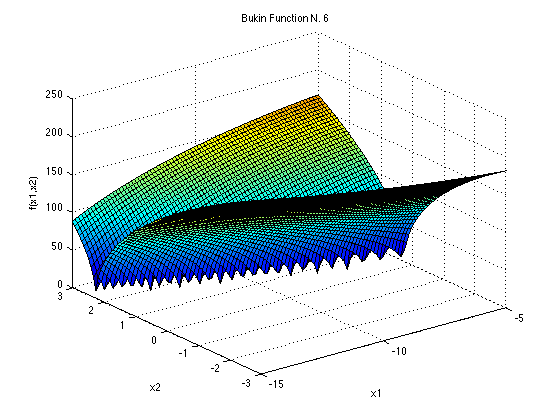
\includegraphics[scale=0.5]{bukin6.png}
    \caption { Gráfico da função Bukin no. 6. }
	\label{fig:bukin6}
\end{center}
\end{figure}

\subsubsection{Função \textit{Ackley}}

A função Ackley é amplamente usada teste de algoritmos de otimização. Em sua forma bidimensional, como mostrada no gráfico abaixo, é caracterizada por uma região externa aparentemente plana e um grande cone no centro. A função possui diversos mínimos locais que podem capturar a atenção dos algoritmos de otimização, especialmente os de escalada.

A expressão da função é a apresentada pela equação \ref{eq:ackley}.

\begin{equation}
	f(x) = -a\ exp\left (-b \sqrt{\frac{1}{d}\sum_{i=1}^{d}x_i^2}\right ) - exp\left (\frac{1}{d}\sum_{i=1}^{d}cos(c x_i)\right ) + a + exp(1)
\label{eq:ackley}
\end{equation}
\\
cuja dimensão é $d$. O domínio de entrada é dado pelo hipercubo $x_i \in [-32.768, 32.768]$ e tem mínimo global em $f(x^*) = 0$, para $x^* = (0,\ldots,0)$. Foram usadas as constantes recomendadas $a = 20$, $b = 0.2$ e $c = 2\pi$.

O gráfico da função é o apresentado na figura \ref{fig:ackley}.
\begin{figure}[htb]
\begin{center}
    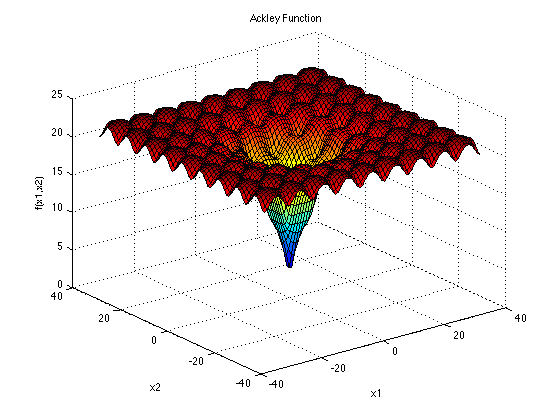
\includegraphics[scale=0.5]{ackley.png}
    \caption { Gráfico da função Ackley. }
    \label{fig:ackley}
\end{center}
\end{figure}

\newpage
\subsubsection{Função \textit{Bohachevsky} no. 1}

As funções Bohachevsky tem, todas, o mesmo formato de cuba.

A expressão da função escolhida é a apresentada pela equação \ref{eq:boha}.

\begin{equation}
	f_1(x) = x_1^2 + 2x_2^2 + -0.3cos(3\pi x_1) - 0.4cos(4\pi x_2) + 0.7 
\label{eq:boha}
\end{equation}
\\
cujo domínio de entrada é dado pelo quadrado $x_i \in [-100, 100]$, para todo $i = 1, 2$ e tem mínimo global em $f_j(x^*) = 0$, para $x^* = (0,0)$, para todo $j = 1, 2, 3$.

O gráfico da função é o apresentado na figura \ref{fig:boha}.

\begin{figure}[htb]
\begin{center}
    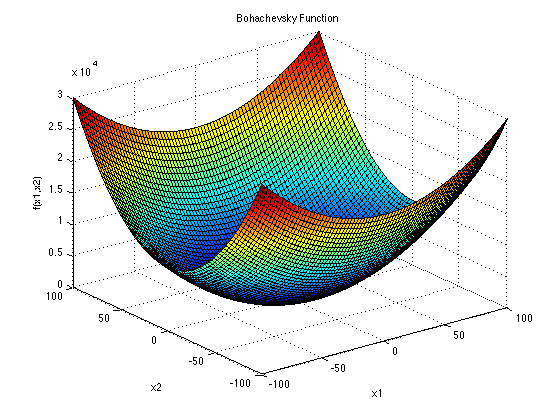
\includegraphics[scale=0.5]{boha.png}
    \caption { Gráfico da função Bohachevsky no. 1. }
    \label{fig:boha}
\end{center}
\end{figure}

%\newpage

%%%%%%%%%%%%%%%%%%%%%% RESULTADOS %%%%%%%%%%%%%%%%%%%%%%%%%%%

\thispagestyle{main}

\section{Resultados}

\subsection{Algoritmo Genético}

Na tabela \ref{table:ga-results} são apresentados os resultados obtidos das médias e desvios-padrão dos melhores indivíduos obtidos após a evolução de 100 gerações para as funções de otimização escolhidas.

\begin{table}[!ht]
\caption{Resultados da otimização com algoritmo genético.}
\label{table:ga-results}
\centering
\begin{tabular}{llclcc}
\toprule
\multicolumn{1}{l}{} & \multicolumn{2}{c}{$x_1$} & \multicolumn{2}{c}{$x_2$} & \multicolumn{1}{c}{} \\
\cmidrule(r){2-3}
\cmidrule(r){4-5}
\multicolumn{1}{l}{Função} & \multicolumn{1}{l}{Intervalo} & \multicolumn{1}{c}{$\bar{\ x_1 }$ \textpm \ $\sigma x_1$} & \multicolumn{1}{c}{Intervalo} & \multicolumn{1}{c}{$\bar{\ x_2 }$ \textpm \ $\sigma x_2$} & \multicolumn{1}{c}{$f(x)$} \\
\midrule
Bukin \#6			& [-15, 5]		& -9,6789 \textpm 1,7845 & [-3, 3]		& 0,9683 \textpm 0,3439 & 0,0434 \textpm 0,2430 \\
Ackley 				& [-40, 40]		& -0,0216 \textpm 0,2605 & [-40, 40]	& 0,0408 \textpm 0,2846 & 0,0434 \textpm 0,2430 \\
Bohachevsky \#1	& [-100, 100]	& -0,0329 \textpm 0,3797 & [-100, 100]	& 0,0065 \textpm 0,2842 & 0,3348 \textpm 1,0575 \\
\bottomrule
\end{tabular}
\end{table}

Os parâmetros utilizados no algoritmo genético, para todas as funções de otimização, foram: população de 100 indivíduos e 100 gerações.

\subsection{Enxame de Partículas}

Na tabela \ref{table:pso-results} são apresentados os resultados obtidos das médias e desvios-padrão das melhores partículas obtidas após a evolução de 50 enxames para as funções de otimização escolhidas.

\begin{table}[!ht]
\caption{Resultados da otimização com enxame de partículas.}
\label{table:pso-results}
\centering
\begin{tabular}{llclcc}
\toprule
\multicolumn{1}{l}{} & \multicolumn{2}{c}{$x_1$} & \multicolumn{2}{c}{$x_2$} & \multicolumn{1}{c}{} \\
\cmidrule(r){2-3}
\cmidrule(r){4-5}
\multicolumn{1}{l}{Função} & \multicolumn{1}{l}{Intervalo} & \multicolumn{1}{c}{$\bar{\ x_1 }$ \textpm \ $\sigma x_1$} & \multicolumn{1}{c}{Intervalo} & \multicolumn{1}{c}{$\bar{\ x_2 }$ \textpm \ $\sigma x_2$} & \multicolumn{1}{c}{$f(x)$} \\
\midrule
Bukin \#6	& [-15, 5]		& -10,3213 \textpm 3,1560 & [-3, 3]		& 1,0653 \textpm 0,6262 & 0	\textpm 0,0163 \\
Ackley		& [-40, 40]		& 7,7230E-11 \textpm 0,2234 & [-40, 40]	& -1,3569E-10 \textpm 0,0816 & 0 \textpm 0,1563 \\
Bohachevsky \#1	& [-100, 100]	& 4,1769E-10 \textpm 0,2241 & [-100, 100]	& -1,0877E-10 \textpm 0,1322 & 0 \textpm 0,1784 \\
\bottomrule
\end{tabular}
\end{table}

Os parâmetros utilizados no enxame de partículas, para todas as funções de otimização, foram: $w = 0.05$, $c_1 = 1.4$, $c_2 = 1.4$, $particulas = 30$ e $enxames = 50$.

%\newpage
%%%%%%%%%%%%%%%%%%%%%%% CONCLUSÃO %%%%%%%%%%%%%%%%%%%%%%%%%%%%

\thispagestyle{main}

\section{Conclusões}

Os resultados obtidos foram consistentes com as informações de solução para as funções escolhidas tendo ambos algoritmos alcançado a convergência necessária para que se pudessem constatar a precisão e a exatidão dos resultados obtidos, corroborando para a conclusão de corretude e prova satisfatória de funcionamento das técnicas.

Observou-se que o algoritmo genético gerou resultados consistentes, mas menos precisos e com velocidade de convergência menor que as obtidas com o enxame de partículas. Pode-se citar como exemplo das observação feita a ordem de grandeza dos resultados de média das soluções obtidas, $x_1$ e $x_2$, que ficaram na casa de $10^{-2}$ para o GA, enquanto que para o PSO ficaram em ordem de grandeza significativamente menor, aproximadamente $10^{-10}$ e $10^{-11}$ nas funções \emph{Ackley} e \emph{Bohachevsky}.

A experiência de implementar e sintonizar as configuraçõe de ambos algoritmos se mostrou mais desafiador para o algortimo genético dada a característica da seleção e do cruzamento, principalmente. As alterações súbtas das informações genéticas das novas populações geravam flutuações inesperadas que levou a equipe a reformular a estratégia de aborgagem do problema de condificação de código genético binário para o modelo de pesos. Já o algoritmo enxame de partículas (PSO) se apresentou mais simples de controlar através dos parâmetros de configuração. A convergência para o valor ótimo da solução ocorreu em todas as execuções do algoritmo.

Comparado com os algoritmos genéricos (GA), o mecanismo de compartilhamento no PSO é substancialmente diferente. No GA, os cromossomos compartilham informações uns com os outros. Portanto, toda a população se move como um grupo em direção a uma área ótima. No PSO, apenas o \emph{\emph{gbest}} presta informações aos demais, assim todas as partículas tendem a convergir para a melhor solução rapidamente, na maioria dos casos.

\newpage

%%%%%%%%%%%%%%%%%%%% REFERÊNCIAS %%%%%%%%%%%%%%%%%%%%%%%%%%%%

\thispagestyle{main}

\begin{thebibliography}{99} % Bibliography 

\bibitem[Linden, 2008]{Linden:2008}
LINDEN, Ricado. (2008).
\newblock {\em Algoritmos genéticos: uma importante ferramenta da Inteligência Computacional}.
\newblock 2a. edição. Rio de Janeiro. Brasport.

\bibitem[Fraser, 1957]{Fraser:1957}
FRASER, Alex. (1957).
\newblock {\em Simulation of genetic systems by automatic digital computers. I. Introduction}.
\newblock Aust. J. Biol. Sci. 10: 484–491.

\bibitem[Fraser, 1970]{Fraser_etal:1970}
FRASER, Alex. BURNELL, Donald. (1970).
\newblock {\em Computer Models in Genetics}.
\newblock New York: McGraw-Hill. ISBN 0-07-021904-4.

\bibitem[Kennedy et al, 1995]{KennedyEberhart:1995}
Kennedy, James, Eberhart, Russell. (1995).
\newblock {\em Particle swarm optimization}. IEEE int'l conf. on neural networks Vol. IV, pp. 1942-1948. IEEE service center, Piscataway, NJ.

\bibitem[Yang et al, 2013]{Yang_etal:2013}
YANG, Xin-She. (2013).
\newblock {\em Swarm Intelligence and Bio-Inspired Computation. Theory and Applications}. 1st. ed. Elsevier.

\bibitem[Moore, 2012]{Moore:2012}
MOORE, Holly. (2012).
\newblock {\em MATLAB ® for engineers}.
\newblock 3rd. edition. Pearson.

\bibitem[Santos, 2013]{Santos:2013}
SANTOS, Tássio Naia dos. (2013).
\newblock LaTeXação. Mais uma apostila de \LaTeX.
\newblock disponível em {\em https://www.ime.usp.br/~tassio/arquivo/latex/apostila.pdf}. acesso em 28/11/2016.

\end{thebibliography}

\appendix

%Apêndice A
\include{apendice}

\end{document}